\section{The heat equation with an explicit Euler}


\chapterDescription
  {
    60 minutes.
  }
  {
    Chapter \ref{chapter:quickstart}.
  }

In this section, we sketch how to realise a heat equation solver for
\[
  \partial _t u - \nabla (\epsilon \nabla) u = 0
\]
that is based
upon an explicit Euler.
It uses the spacetree as computational grid.


\subsection{Preparation}

We create an empty project with the PDT (\texttt{--create-project myproject
myproject}) and first adopt our cell and vertex data structure such that each
cell holds an $\epsilon$ value and each vertex holds the current and previous
solution.

\begin{code}
Packed-Type: short int;
class myproject::dastgen::Vertex {
  parallelise persistent double  u;
  discard                double  oldU;
};
\end{code}


\begin{code}
Packed-Type: short int;
class myproject::dastgen::Cell {
  persistent double epsilon;
};
\end{code}


\noindent
Furthermore, we make the code's state hold the solver's time step size. We will
write the code such that it works in 2d and 3d. All the pictures are done for a
3d setup. To run with other dimensions, you have to adopt your makefile
accordingly.


\begin{code}
Packed-Type: short int;
class myproject::dastgen::State { 
  persistent parallelise double dt;
};
\end{code}


\noindent
We do not use any sophisticated plotting routines and thus rely in some plotters
that are available out-of-the-box for Peano.
We also require only two mappings: one for the setup, one for the time stepping. 
Depending on our personal choices, we combine them with plotting features or
not\footnote{There is a known issue with the coding standards in Peano/PDT
which can be avoided a priori if all read and write attributes start with an
uppercase---even though they might be defined with lowercase in the def file.}.

\begin{code}
omponent: ExplicitEulerForHeatEquation
namespace: ::myproject
vertex:
  dastgen-file: Vertex.def
  read scalar(double): U
  read scalar(double): OldU
  write scalar(double): U
cell:
  dastgen-file: Cell.def
state:
  dastgen-file: State.def
event-mapping:
  name: CreateGrid
event-mapping:
  name: TimeStep
adapter:
  name: CreateGrid
  merge-with-user-defined-mapping: CreateGrid
adapter:
  name: TimeStep
  merge-with-user-defined-mapping: TimeStep
adapter:
  name: CreateGridAndPlot
  merge-with-user-defined-mapping: CreateGrid
  merge-with-predefined-mapping: VTKPlotCellValue(epsilon,getEpsilon,eps)
  merge-with-predefined-mapping: VTKPlotVertexValue(initialSetup,getU,u)
adapter:
  name: TimeStepAndPlot
  merge-with-user-defined-mapping: TimeStep
  merge-with-predefined-mapping: VTKPlotVertexValue(result,getU,u)
\end{code}

\noindent
To translate this file, you need the corresponding predefined mappings that are 
held in the repository or on the webpage.
To find out what the arguments of the predefined mappings mean, please have a 
look into the corresponding template header files.
We note that we write out epsilon only throughout the setup phase. 
It does not make sense to plot each each iteration, as this material parameter
does not change in time.
We furthermore note that we add some \texttt{read} and \texttt{write}
statements.
They make the PDT generate helper methods that allow us within each cell to
access all $u$ values of a cell as one vector.



\subsection{Making the plotter work}

This code so far does not compile. It complains with

\begin{code}
> make -f myproject/makefile
--- This is Peano 3 ---
g++ -DDim3 [...] -c myproject/adapters/CreateGridAndPlot2VTKPlotCellValue_0.cpp -o \
myproject/adapters/CreateGridAndPlot2VTKPlotCellValue_0.o 
[...]  In member function ‘void [...]::CreateGridAndPlot2VTKPlotCellValue_0::enterCell([...])’:
[...] error: ‘class myproject::Cell’ has no member named ‘getEpsilon’
     _cellValueWriter->plotCell(cellIndex,fineGridCell.getEpsilon() );
                                                       ^
make: *** [myproject/adapters/CreateGridAndPlot2VTKPlotCellValue_0.o] Error 1
\end{code}

\noindent
This is correct. 
We have told the predefined mapping that there would be an opteration
\texttt{getEpsilon} to print cell data, but we have not provided one yet.
A similar reasoning holds for the plotting of the actual solution.
Therefore, we add 

\begin{code}
void myproject::Cell::init() {
  _cellData.setEpsilon( 1.0 + static_cast<double>(rand() % 100)/100.0 );
}

double myproject::Cell::getEpsilon() const {
  return _cellData.getEpsilon();
}
\end{code}

\noindent
This snippet also allows us to initialise a cell with a random value from
$(1,2)$.


\begin{remark}
An initialisation of the cell's $\epsilon$ in the default constructor does not
work because of the flyweight pattern (see next remark). Instead, we have to
provide an explicit initialisation routine, and we have to call this routine
within the mapping's \texttt{createCell} event.
\end{remark}

\noindent
We reiterate our code extension for the vertex,

\begin{code}
double myproject::Vertex::getU() const {
  return _vertexData.getU();
}
\end{code}

\noindent
Finally, we plug into \texttt{CreateGrid}'s \texttt{createInnerVertex} and
\texttt{createBoundaryVertex} and add some refinement statements:

\begin{code}
void myproject::mappings::CreateGrid::createInnerVertex(...) {
 if (coarseGridVerticesEnumerator.getLevel()<4) {
  fineGridVertex.refine();
 }
} 
 
void myproject::mappings::CreateGrid::createBoundaryVertex(...) {
 if (coarseGridVerticesEnumerator.getLevel()<4) {
  fineGridVertex.refine();
 }
} 
 
void myproject::mappings::CreateGrid::createCell(...) {
 logTraceInWith4Arguments( "createCell(...)", fineGridCell, ... );

 fineGridCell.init();

 logTraceOutWith1Argument( "createCell(...)", fineGridCell );
}
  
\end{code}

As soon as this first plot is available, as add a time stepping loop in the
\texttt{runners::Runner}:

\begin{code}
int myproject::runners::Runner::runAsMaster(myproject::repositories::Repository& repository) {
  peano::utils::UserInterface userInterface;
  userInterface.writeHeader();

  repository.switchToCreateGridAndPlot();
  repository.iterate();
  
  repository.getState().setTimeStepSize( 1e-7 );
  for (int i=0; i<1000; i++) {
    if (i%10==0) {
      repository.switchToTimeStepAndPlot();
    }
    else {
     repository.switchToTimeStep();
    }
    repository.iterate();
  }
 
  repository.logIterationStatistics();
  repository.terminate();

  return 0;
}
\end{code}

\noindent
The implementation of the \texttt{State}'s \texttt{void setTimeStepSize(double
dt)} operation is left to the reader. 
Please add the corresponding \texttt{double getTimeStepSize() const}, too.

\begin{center}
  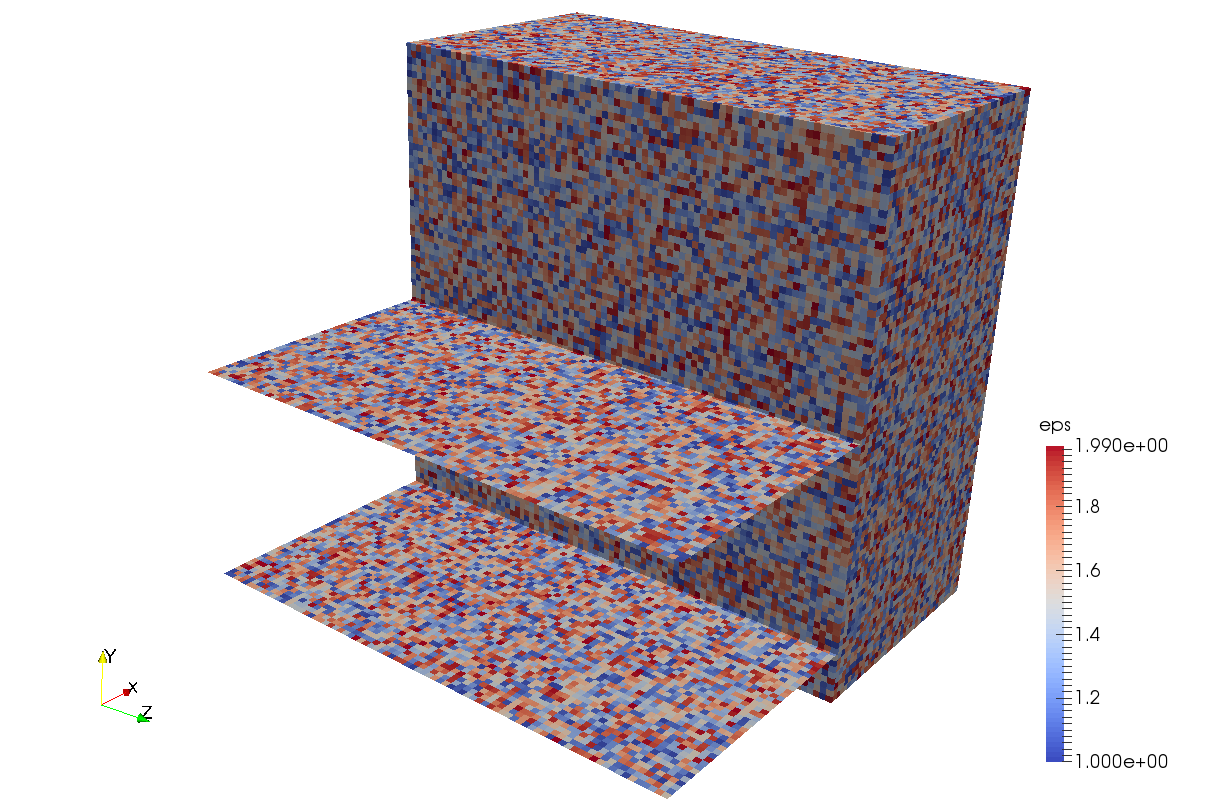
\includegraphics[width=0.7\textwidth]{41_heat-equation/epsilon.png}
\end{center}



\begin{remark}
  It is a `original' decision to model states, vertices and cells as classes
  that actually aggregate their data objects (attribute \texttt{\_stateData},
  \texttt{\_vertexData} or \texttt{\_cellData}, respectively).
  The reason for this is two-fold:
  On the one hand, this allows us to separate user-defined code (the
  aggregating class) from the data model generated by DaStGen. The latter also
  comprises complex technical details such as the MPI data types or bit
  compression. If application-specific code is rewritten, the data model is not
  affected and the other way round. On the other hand, the pattern allows us to
  apply the flyweight pattern. A vertex object is not actually stored and loaded
  from input data. It exists only a few time in total, and in each step its
  change is exchanged underneath by the traversal.
\end{remark}




\subsection{A stencil code}

In this example, we stick to a finite differences formulation and
vertex-centred unknown assignment to do the time stepping.
Our strategy (within the mapping) is simple:
\begin{enumerate}
  \item In \texttt{beginIteration}, we grab the time step size from the state.
  This way, the user might alter the time step size in the outer control loop
  (adaptive time stepping).
  The mapping then always works with the right parameter.
  \item In \texttt{touchVertexFirstTime}, we take the current solution and back
  it up in the vertex's property \texttt{\_oldU}. This property is marked as
  discard, i.e.~the additional helper variable per vertex is not held in-between
  two iterations (actually it is only held for a small number of vertices that
  are still in use). 
  \item In \texttt{enterCell}, we element-wisely accumulate the new solution in
  the vertices.
\end{enumerate}

\begin{code}
class myproject::mappings::TimeStep {
 private:
  /**
   * Logging device for the trace macros.
   */
  static tarch::logging::Log  _log;
    
  double _timeStepSize;
  ...
};


void myproject::mappings::TimeStep::beginIteration(
  myproject::State&  solverState
) {
  logTraceInWith1Argument( "beginIteration(State)", solverState );

  _timeStepSize = solverState.getTimeStepSize();

  logTraceOutWith1Argument( "beginIteration(State)", solverState);
}
\end{code}

\noindent
We reiterate that the state is not available to a mapping by default. If you
need the state (or one of its properties), you explicitly have to grab this data
in \texttt{beginIteration}. As an alternative to the double above, it also would
be possible to copy the whole state. If you want to modify the solver's state,
you have to alter it in \texttt{endIteration}. As Peano requires the user to
explicitly move state data around when required, we ensure that the data remains
consistent in the parallel code variants.

\begin{code}
void myproject::mappings::TimeStep::touchVertexFirstTime(...) {
 ...  
 fineGridVertex.copyCurrentSolutionIntoOldSolution();
 ...  
}

void myproject::Vertex::copyCurrentSolutionIntoOldSolution() {
  _vertexData.setOldU( _vertexData.getU() );
}
\end{code}

\noindent
The interesting stuff happens in the mapping's \texttt{enterCell}, 
where we first of all take all $2^d$ vertices and write their old solution into
one double vector. 
For this, there's a predefined operation in \texttt{VertexOperations} as we have
asked the PDE that we read the scalar.
This $2^d$ vector then is multiplied with the local assembly matrix subject of
an $\epsilon$ scaling.
The result finally is added to the new value.
Again, we us the generated read and write methods.

\begin{code}
#include "myproject/VertexOperations.h"
#include "tarch/la/Matrix.h"

void myproject::mappings::TimeStep::enterCell(...) {
  logTraceInWith4Arguments( "enterCell(...)", fineGridCell, ... );

  tarch::la::Matrix<TWO_POWER_D,TWO_POWER_D,double> A;

  A =  1.0, -0.5, -0.5,  0.0, -0.5,  0.0,  0.0,  0.0,
      -0.5,  1.0,  0.0, -0.5,  0.0, -0.5,  0.0,  0.0,
      -0.5,  0.0,  1.0, -0.5,  0.0,  0.0, -0.5,  0.0,
       0.0, -0.5, -0.5,  1.0,  0.0,  0.0,  0.0, -0.5,
      -0.5,  0.0,  0.0,  0.0,  1.0, -0.5, -0.5,  0.0,
       0.0, -0.5,  0.0,  0.0, -0.5,  1.0,  0.0, -0.5,
       0.0,  0.0, -0.5,  0.0, -0.5,  0.0,  1.0, -0.5,
       0.0,  0.0,  0.0, -0.5,  0.0, -0.5, -0.5,  1.0;

  tarch::la::Vector<TWO_POWER_D,double> uOld = 
    VertexOperations::readOldU(fineGridVerticesEnumerator,fineGridVertices);

  const double h = fineGridVerticesEnumerator.getCellSize()(0);

  tarch::la::Vector<TWO_POWER_D,double> uUpdate = 
    - _timeStepSize * fineGridCell.getEpsilon() * A * uOld / h / h  ;

  VertexOperations::writeU(
    fineGridVerticesEnumerator,fineGridVertices,
    VertexOperations::readU(fineGridVerticesEnumerator,fineGridVertices) + uUpdate
  );

  logTraceOutWith1Argument( "enterCell(...)", fineGridCell );
}
\end{code}

\noindent
In this example, I wrote down the local assembly matrix for $d=3$ explicitly.
If you want to support other dimensions, you have to adopt this part
accordingly.
Alternatively, you might want to use Peano's dimension-generic tools and write
one-version-fits-it-all.

We use Peano's linear algebra routines here.
They are held in the \texttt{tarch} component, and provide all basic
functionality we typically need.
Obviously, it might make sense to switch to other linear algebra packages
(BLAS, e.g.) for more demanding setups.

For a better understanding, it might make sense to have a look into
\texttt{readOldU}.
We note that \texttt{fineGridVertices} is a pointer to an array of vertices, but
the layout of the vertices within this array remains open.
Therefore, Peano hands over an enumerator object. 
The enumerator object has a functor to allow us to select the right vertices.
\texttt{fineGridVertices[ fineGridVerticesEnumerator(0) ]} for example returns
the bottom left vertex of the cell.
See the enumerator's documentation in the header for detailed information.
The read and write that are generated by the PDT run through the vertices and
collect the \texttt{u} or \texttt{oldU} value, respectively, in one vector.
They are scatter/gather operations.
Some codes might prefer not to rely on the temporary vectors and instead work
with the data associated to the vertices directly.
Both options are fine, both options might have different performance
characteristics.

 
Obviously, the above code is not very elaborate. 
The stiffness matrix is set up multiple times.
The most basic optimisation would be to make the matrix an attribute of the
mapping and to initialise it only once.

\begin{remark}
  On the Peano webpage and in the repository, you find a \texttt{matrixfree}
  toolbox. It contains all kind of primitive helper operations that allow you to
  work with stencil codes. It is not as powerful as a real stencil compiler or 
  other matrix-free/PDE toolboxes, but it a small suite to build up at least the
  simpler PDE operators from a finite element/tensor-product formalism and it
  also provides operations fitted to PDT's generated read and write routines. 
\end{remark}


\noindent
Obviously, our code does not do anything as we do not set any nonzero boundary
conditions. 
Lets do this upon a vertex's first use. 
As we have specified a read, the PDT provides write operations that break up the
object encapsulation.
We make use of this now:

\begin{code}
void myproject::mappings::TimeStep::touchVertexFirstTime(...) {
  ...
  if (fineGridVertex.isBoundary() && fineGridX(0)<1e-8) {
    VertexOperations::writeU( fineGridVertex, 1.0 );
  }
  else if (fineGridVertex.isBoundary()) {
    VertexOperations::writeU( fineGridVertex, 0.0 );
  }
  ...
}
\end{code}

\begin{center}
  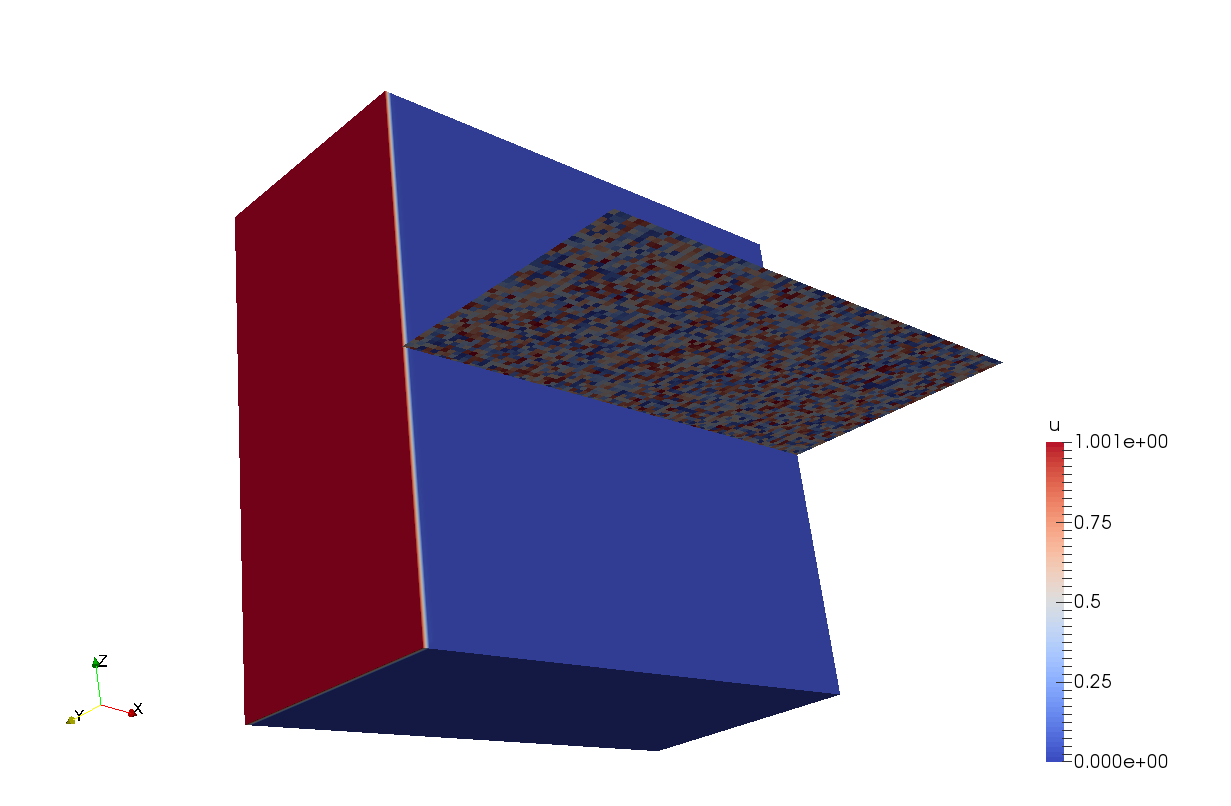
\includegraphics[width=0.45\textwidth]{41_heat-equation/solution00.png}
  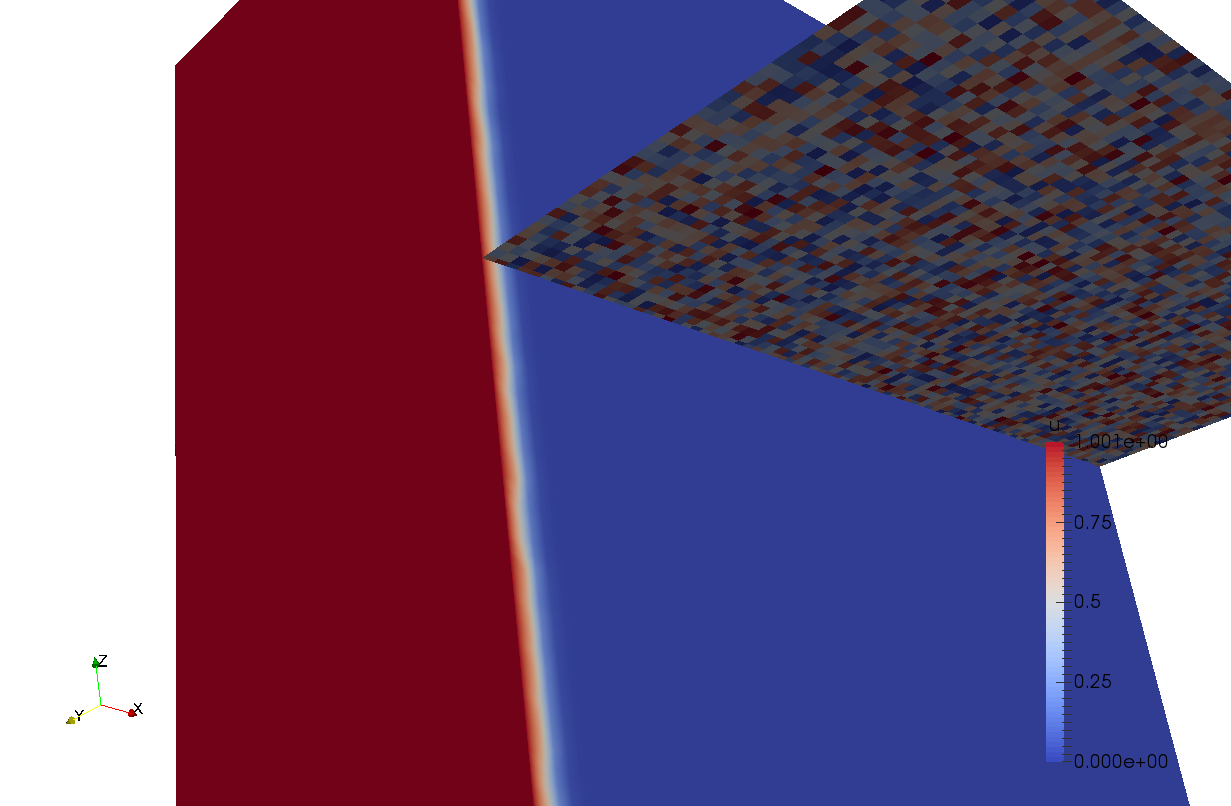
\includegraphics[width=0.45\textwidth]{41_heat-equation/solution01.png}
  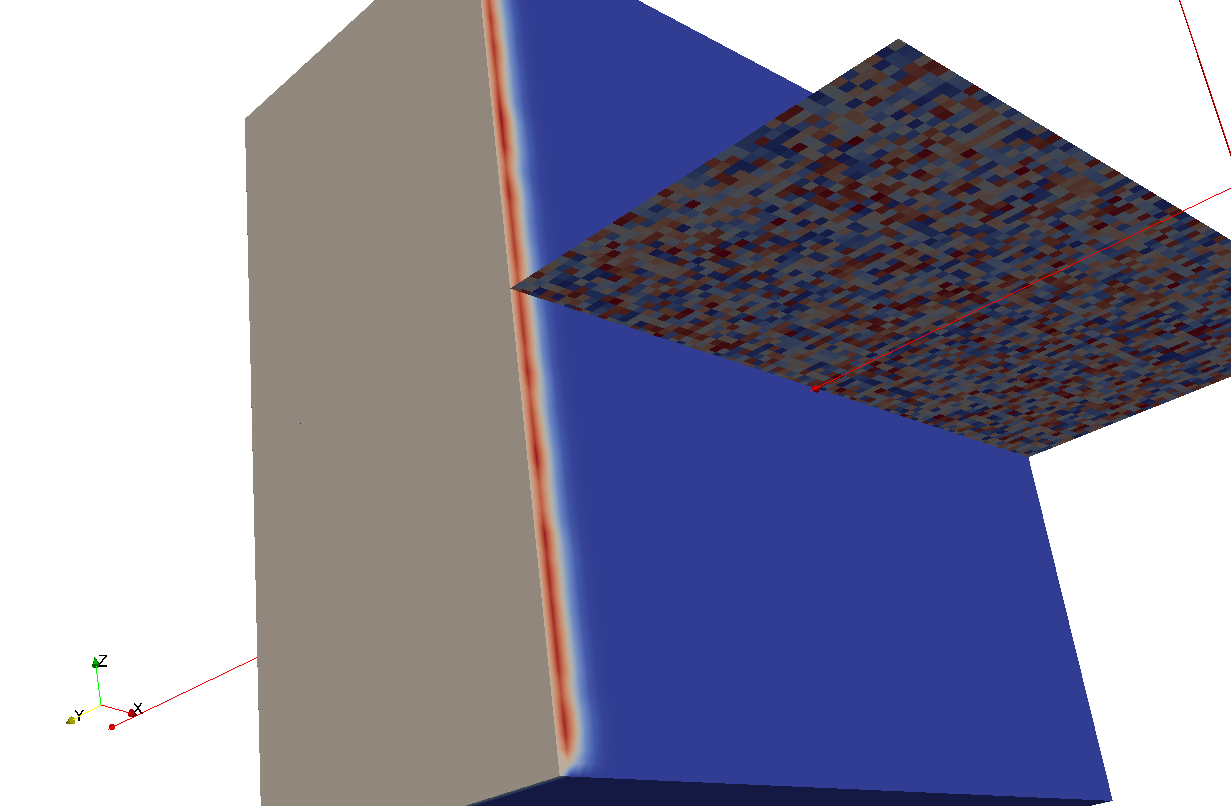
\includegraphics[width=0.45\textwidth]{41_heat-equation/solution02.png}
  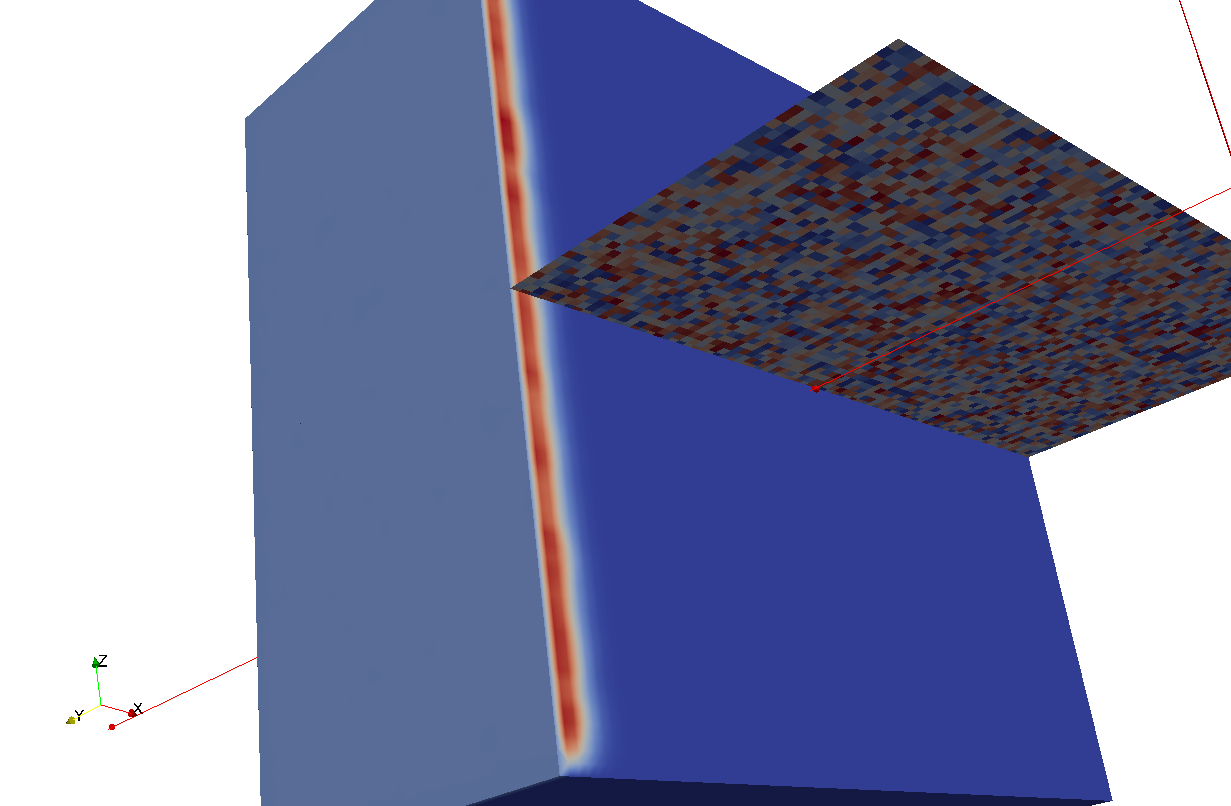
\includegraphics[width=0.45\textwidth]{41_heat-equation/solution03.png}
\end{center}


All figures cut through the domain in the middle and use an orthogonal slice to
visualise the permeability $\epsilon$.
Top, left: We start from a zero condition where only the face at $x=0$ is set to
$1$.
Top, right: Very slowly, the temperature propagates through the domain. As
$\epsilon $ is fuzzy, the propagation profile does not exhibit symmetry but is
ragged as well.
Bottom: The temperature propagates further into the medium.


\subsection{Static adaptivity}



% Noch was zu FAC
%injection


\subsection{Dynamic adaptivity}
